\documentclass[10pt, xcolor={usenames, dvipsnames, table}]{beamer}
%\documentclass[handout, 10pt, xcolor={usenames, dvipsnames}]{beamer}

\usepackage{etex}
\usepackage[english]{babel}
\usepackage[utf8]{inputenc}
\usepackage[T1]{fontenc}
\usepackage{amsfonts}
\usepackage{amsmath}
\usepackage{amssymb}
\usepackage{graphicx}
\usepackage{hyperref}
\usepackage{booktabs}
\usepackage[round]{natbib}
\usepackage{tikz}
\usepackage{colortbl}
\usepackage{ulem}
\usepackage{multicol}
\usepackage[overlay]{textpos}
\usepackage{multirow}
\usepackage{ifthen}
\usepackage{ragged2e}
\usepackage{rotating}
\usepackage{pgfplots}
\usepackage{fancybox}
\usepackage{ulem}
\usepackage{overpic}
\usepackage{enumerate}
\usepackage{xfrac}

\setcounter{tocdepth}{2}

\usetheme[style=lina]{min}

\pgfplotsset{compat=1.8}
\usetikzlibrary{positioning, topaths, shapes, arrows, patterns, calc}
\newcount\mycount
\tikzstyle{io}=[
  ellipse,
  minimum width=5cm,
  minimum height=2cm,
  fill=linagreen!30,
  draw=linagreen!40,
  transform shape,
  font={\huge}
]
\tikzstyle{selectedio}=[
  io,
  fill=linared!30,
  draw=linared!40,
]
\tikzstyle{component}=[
  thick,
  rectangle,
  minimum width=13cm,
  minimum height=2cm,
  text centered,
  text width=12.5cm,
  fill=Cerulean!20,
  draw=Cerulean!30,
  transform shape,
  font={\huge\bfseries}
]
\tikzstyle{selectedcomponent}=[
  component,
  fill=linared!30,
  draw=linared!40,
]

\title{Keyphrase Annotation\\with Graph Co-Ranking}
\author{
  \textbf{Adrien \textsc{Bougouin}},
  Florian \textsc{Boudin},
  Béatrice \textsc{Daille}
 }
\institute{Université de Nantes, LINA}
\date{December 16$^{\textnormal{th}}$, 2016}
\titlepageextra{
  \vfill{}
  \includegraphics[height=6em]{logo/coling_2016.png}
  \vfill{}
}
\logos{
  \hfill{}\includegraphics[height=2.4em]{logo/univ_nantes.eps}
  \hfill{}
\includegraphics[height=2.4em]{logo/lina.eps}
  \hfill{}\includegraphics[height=2.4em]{logo/termith.eps}
  \hfill{}
}

\makeatletter
\def\rowcolor{\noalign{\ifnum0=`}\fi\bmr@rowcolor}
\newcommand<>{\bmr@rowcolor}{%
    \alt#1%
        {\global\let\CT@do@color\CT@@do@color\@ifnextchar[\CT@rowa\CT@rowb}% 
        {\ifnum0=`{\fi}\@gooble@rowcolor}% 
}

\newcommand{\@gooble@rowcolor}[2][]{\@gooble@rowcolor@}
\newcommand{\@gooble@rowcolor@}[1][]{\@gooble@rowcolor@@}
\newcommand{\@gooble@rowcolor@@}[1][]{\ignorespaces}
\makeatother



\makeatletter
\def\cellcolor{{\ifnum0=`}\fi\bmr@cellcolor}
\newcommand<>{\bmr@cellcolor}{%
    \alt#1%
        {\global\let\CT@do@color\CT@@do@color\@ifnextchar[\CT@rowa\CT@rowb}% 
        {\ifnum0=`{\fi}\@gooble@cellcolor}% 
}

\newcommand{\@gooble@cellcolor}[2][]{\@gooble@cellcolor@}
\newcommand{\@gooble@cellcolor@}[1][]{\@gooble@cellcolor@@}
\newcommand{\@gooble@cellcolor@@}[1][]{\ignorespaces}
\makeatother

\begin{document}
  \begin{frame}[plain, noframenumbering]
    \titlepage
  \end{frame}
  
  \section{Introduction}
\label{sec:section}
    Keyphrases are words or phrases that represent the main content of a document.
    Similar to an abstract, keyphrases give a synoptic picture of what is important in the document.
    Disimilar to an abstract, keyphrases are small grain units and are useful resources for many Natural Language Processing tasks: document clustering~\cite{han2007webdocumentclustering}, information retrieval~\cite{medelyan2008smalltrainingset}, document summarization~\cite{litvak2008graphbased}, etc.
    However, documents do not always contain keyphrases.
    As the daily flow of new documents grows, manually annotating documents has become impractical.
    Hence automatic keyphrase extraction recently attracts a lot of attention and many different methods are proposed~\cite{hasan2014state_of_the_art}.

    Automatic keyphrase extraction is the task of detecting important words or phrases within a document.
    Generally speaking, we divide keyphrase extraction methods into two categories: supervised and unsupervised.
    Supervised methods treat keyphrase extraction as a binary classification task, e.g.~\cite{witten1999kea}.
    Conversely, unsupervised methods usually rank keyphrase candidates by importance and select the top-ranked ones as keyphrases, e.g.~\cite{mihalcea2004textrank}.

    Although they tackle the keyphrase extraction problem differently, both supervised and unsupervised methods rely on a candidate selection step.
    Keyphrase candidate selection identifies words or phrases consistent with human-assigned keyphrase properties.
    %Although keyphrase candidate selection starts to draw attention~\cite{wang2014keyphraseextractionpreprocessing}, keyphrase extraction methods use simple heuristics: selection of n-grams, sequences of nouns and adjectives, etc.
    However, current selection methods use simple heuristics~\cite{wang2014keyphraseextractionpreprocessing}: candidates are n-grams or sequences of nouns and adjectives.
    %This work infers linguistic properties from human-assigned keyphrases and demonstrates their applicability on keyphrase candidate selection.
    This work proposes rules based on a comprehensive analysis of modifiers within human-assigned keyphrases.
    We demonstrate their applicability on keyphrase candidate selection.
    
    This paper is organized as follows.
    Section~\ref{sec:keyphrase_properties} presents an analysis of human-assigned keyphrases.
    Section~\ref{sec:candidate_selection} describes common keyphrase candidate selection methods followed by a description of our method in Section~\ref{sec:proposed_candidate_selection_method}. Finally, Section~\ref{sec:experiments} presents the expriments and Section~\ref{sec:conclusion} concludes our work.

  \begin{frame}{Outline}
    \tableofcontents
  \end{frame}
  \section{Related Work}
\label{sec:related_work}
  \TODO{Introduction to the standard pipeline}

  \subsection{Automatic Keyphrase Extraction}
  \label{subsec:ake}
    \begin{itemize}
      \item{TF-IDF, Likey, etc.}
      \item{Graph-based methods (focus on TopicRank)}
      \item{GenEX, KEA, HUMB, etc. (focus on KEA)}
    \end{itemize}

  \subsection{Automatic Keyphrase Assignment}
  \label{subsec:aka}
    \begin{itemize}
      \item{KEA++ (Automatic Keyphrase Indexing)}
      \item{WAM (SMT AKA method)}
    \end{itemize}

  \subsection{Graph co-ranking for NLP}
  \label{subsec:graph_co_ranking_for_nlp}
    \begin{itemize}
      \item{Xiaojun Wan: Cross-language document summarization}
      \item{Rui Yan: Tweet recommendation}
      \item{Kang Liu: Opinion mining (check) from online reviews}
    \end{itemize}


  \AtBeginSection[]{
    \begin{frame}{Outline}
      \tableofcontents[currentsection]
    \end{frame}
  }
  \section{Proposal}
\begin{frame}{Proposal}
  \begin{figure}
    \centering
    \begin{tikzpicture}[scale=.35, node distance=3cm]
      \node [component, minimum width=29cm, text width=28cm] (extraction_assignment) {Keyphrase Extraction \hspace{4.25em} \& \hspace{3.66em} Keyphrase Assignment};
  
      \node [io, above=of extraction_assignment, xshift=-8cm] (document) {document};
      \node [io, above=of extraction_assignment, xshift=8cm] (controlled_vocabulary) {controlled vocabulary};
  
      \node [io, below=of extraction_assignment] (keyphrases) {keyphrases $\subseteq$ document $\cup$ controlled vocabulary};
  
      \draw [dashed] ($(extraction_assignment.north west)+(-.5cm, 5.5cm)$) rectangle ($(extraction_assignment.south east)+(1cm, -5.5cm)$);
      \node [above=of document, yshift=-2.9cm, xshift=2.75cm] (document_centric) {\small keyphrase annotation};
  
      \path [->] (document) edge (extraction_assignment);
      \path [->] (extraction_assignment) edge (keyphrases);
      \path [->] (controlled_vocabulary) edge (extraction_assignment);
    \end{tikzpicture}
  \end{figure}
\end{frame}


  \begin{frame}{Contributions}\framesubtitle{TopicCoRank}
  \begin{alertblock}{TODO}
    \begin{itemize}
      \item{Extension supervisée de TopicRank}
      \item{Adaptaion en domaines de spécialité}
      \item{$\Rightarrow$ Assignement}
      \item{Problèmes identifiés de l'assignement}
    \end{itemize}
  \end{alertblock}
\end{frame}

\begin{frame}{TopicCoRank}\framesubtitle{Proposition}
\end{frame}

\begin{frame}{TopicCoRank}\framesubtitle{Exemple}
\end{frame}

\begin{frame}{TopicCoRank}\framesubtitle{Évaluation}
\end{frame}

\begin{frame}{TopicCoRank}\framesubtitle{Résultats}
\end{frame}

\begin{frame}{TopicCoRank}\framesubtitle{Bilan}
\end{frame}


  \section{Experimental Settings}
\label{sec:experimental_settings}
  \subsection{Dataset}
  \label{subsec:dataset}
    In this work, we use the SemEval corpus. Built for the task 5 of
    SemEval-2010~\cite{kim2010semeval}, Sem\-Eval contains 244 English
    scientific papers collected from the ACM Digital Libraries. We use
    Sem\-Eval's training set (144 documents) and test set (100 documents) with
    their sets of combined author- and reader-assigned keyphrases.

  \subsection{Baselines}
  \label{subsec:baselines}
    In order to show that our method benefits from all aspects of its
    configuration, we design a set of baselines that slightly diverge from our
    method (derived baselines). First, To\-picRank plus the SVM classifier
    trained on either candidate- and cluster-based features (TopicRank+SVM),
    while the SVM classifier is trained on all features for our method
    (TopicRank+SVM$_{\text{all}}$). Second the SVM classifier, trained on either
    candidate-based, cluster-based or all features, is applied to the unranked
    clusters (Clustering+SVM). Finally, the SVM classifier, trained on
    candidate-based features, is applied to the candidate keyphrases (SVM).

    For comparison purpose, we also report results of a Naive Bayes classifier
    trained with the first position and the TF-IDF
    features~\cite[KEA]{witten1999kea}, TF-IDF and TopicRank.

  \subsection{Preprocessing}
  \label{subsec:preprocessing}
    For our method, as well as all baselines, we use Topic\-Rank's
    outputs. %\footnote{Outputs of TopicRank can be obtained from sources at:
    %\url{http://git.io/topicrank_ijcnlp_2013}.}.
    Therefore, our results can directly be compared to results
    in~\cite{bougouin2013topicrank}.

  \subsection{Evaluation Measures}
  \label{subsec:evaluation_measures}
    We evaluate the performance of our method and the baselines in terms of
    precision (P), recall (R) and f-score (f1-measure, F) when at most 10
    keyphrases are extracted. In order to reduce mismatches due to flexions such
    as plural, we also stem candidate and reference keyphrases during the
    evaluation.

\section{Results}
\label{sec:results}
  \begin{figure}
    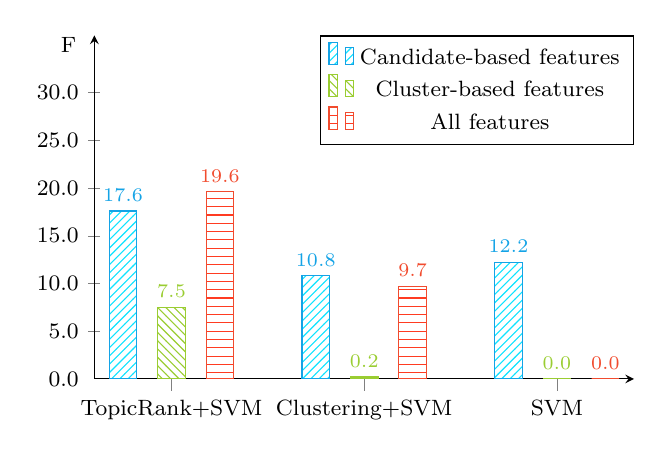
\begin{tikzpicture}
      \pgfkeys{/pgf/number format/.cd, fixed, fixed zerofill, precision=1}
      \begin{axis}[axis lines=left,
                   symbolic x coords={TopicRank+SVM, Clustering+SVM, SVM},
                   xtick=data,
                   enlarge x limits=0.2,
                   xticklabel style={font=\footnotesize},
                   nodes near coords,
                   nodes near coords align={vertical},
                   every node near coord/.append style={font=\scriptsize},
                   ytick={0.0, 5.0, 10.0, 15.0, 20.0, 25.0, 30.0},
                   yticklabel style={font=\footnotesize},
                   y=0.01\linewidth,
                   ymin=0.0,
                   ymax=36.0,
                   ybar=7.5pt,
                   ylabel=F,
                   ylabel style={at={(ticklabel* cs:1)},
                                 anchor=north east,
                                 yshift=.3em,
                                 xshift=.3em,
                                 rotate=270,
                                 font=\footnotesize},
                   legend style={at={(1.0, 1.0)},
                                 anchor=north east,
                                 font=\footnotesize}]
        \addplot[Cerulean,
                 pattern=north east lines,
                 pattern color=Cerulean] coordinates{
          (SVM, 12.2)
          (Clustering+SVM, 10.8)
          (TopicRank+SVM, 17.6)
        };
        \addplot[YellowGreen,
                 pattern=north west lines,
                 pattern color=YellowGreen] coordinates{
          (SVM, 0.0)
          (Clustering+SVM, 0.2)
          (TopicRank+SVM, 7.5)
        };
        \addplot[RedOrange,
                 pattern=horizontal lines,
                 pattern color=RedOrange] coordinates{
          (SVM, 0.0)
          (Clustering+SVM, 9.7)
          (TopicRank+SVM, 19.6)
        };
        \legend{Candidate-based features, Cluster-based features, All features}
      \end{axis}
    \end{tikzpicture}
    \caption{Performance of TopicRank+SVM$_{\text{all}}$ compared to derived
             baselines
             \label{fig:baseline_comparison}}
  \end{figure}

  Figure~\ref{fig:baseline_comparison} presents the performance of our method,
  compared to six baselines derived from it. On the first hand, we observe that
  using clusters and their importance score benefits to the keyphrase
  extraction. Most importantly, adding cluster-based features to the common
  features (candidate-based features) improves the performance. However, the
  performance achieved with the Clustering+SVM method shows that cluster-based
  features performs poorly when Topic\-Rank's importance score is not used.
  Additionally, the SVM performance tends to show that using clusters without
  taking their importance into account is not relevant. Results support our
  assumption that keyphrases should be extracted from important topics.

  \begin{table}
    \centering
    \begin{tabular}{|r|rrr|}
      \hline
      Method & \multicolumn{1}{c}{P} & \multicolumn{1}{c}{R} & \multicolumn{1}{c|}{F}\\
      \hline
      KEA                           & 18.8\textcolor{white}{$^\dagger$} & 13.3\textcolor{white}{$^\dagger$} & 15.4\textcolor{white}{$^\dagger$}\\
      TF-IDF                        & 13.2\textcolor{white}{$^\dagger$} & 8.9\textcolor{white}{$^\dagger$} & 10.5\textcolor{white}{$^\dagger$}\\
      TopicRank                     & 14.9\textcolor{white}{$^\dagger$} & 10.3\textcolor{white}{$^\dagger$} & 12.1\textcolor{white}{$^\dagger$}\\
      TopicRank+SVM$_{\text{all}}$  & 24.2$^\dagger$ & 16.7$^\dagger$ & 19.6$^\dagger$\\
      \hline
      TopicRank$_{\text{max}}$      & 37.6\textcolor{white}{$^\dagger$} & 25.8\textcolor{white}{$^\dagger$} & 30.3\textcolor{white}{$^\dagger$}\\
      \hline
    \end{tabular}
    \caption{Performance of TopicRank+SVM$_{\text{all}}$ compared to previous
             work. $\dagger$ indicates improvement over KEA, TF-IDF and
             TopicRank at 0.001 level using Student's t-test.
             \label{tab:state_of_the_art_comparison}}
  \end{table}

  Also, Table~\ref{tab:state_of_the_art_comparison} presents a comparison of
  TopicRank+SVM$_{\text{all}}$ with TopicRank, TopicRank's best possible
  performance (TopicRank$_{\text{max}}$) and common baselines of previous work.
  Results show that our method significantly improves TopicRank and
  significantly outperforms TF-IDF and KEA, a robust supervised methods.
  However, the performance of TopicRank+SVM$_{\text{all}}$ is still very low
  compared to TopicRank$_{\text{max}}$. The naivety of the clustering method
  TopicRank applies may introduce noise that dampens the performance. Future
  improvement should focus on a more efficient clustering of the candidates
  belonging to the same topic.

%\section{Example}
%\label{sec:example}


  \section{Conclusion et perspectives}
\label{sec:conclusion_et_perspectives}
  Dans ce travail, nous proposons une méthode à base de graphe pour l'extraction
  non supervisée de termes-clés. Cette méthode groupe les termes-clés candidats
  en sujets, détermine quels sont ceux les plus importants, puis extrait le
  terme-clé candidat qui représente le mieux chacun des sujets les plus
  importants. Cette nouvelle méthode offre plusieurs avantages vis-à-vis des
  précédentes à base de graphe. Le groupement des termes-clés potentiels en
  sujets distincts permet de rassembler des indices utiles auparavant éparpillés
  et le choix d'un seul terme-clé pour représenter un sujet important permet
  d'extraire un ensemble de termes-clés non redondants ( pour $k$ termes-clés
  extraits, exactement $k$ sujets sont couverts). Enfin, le graphe est complet
  et ne requiert plus le paramétrage d'une fenêtre de cooccurrences,
  contrairement aux autres méthodes à base de graphe.

  Les bons résultats de notre méthode montrent la pertinence d'un groupement en
  sujets des candidats pour ensuite les ordonner. Les expériences
  supplémentaires montrent aussi qu'il est encore possible d'améliorer notre
  méthode en proposant une nouvelle stratégie de sélection du terme-clé candidat
  le plus représentatif d'un sujet (pour un gain maximum allant de 4,2 à 15
  points de f-score).

  Nous avons aussi effectué une analyse d'erreurs à partir de laquelle trois
  perspectives de travaux futurs émergent~:

  Nous avons pour objectif d'améliorer la sélection des termes-clés candidats.
  Aussi, des méthodes empruntées à d'autres domaines du TAL peuvent être
  appliquées. Il semble, par exemple, pertinent d'évaluer l'apport des méthodes
  d'extraction terminologiques~\cite{castellvi2001automatictermdetection} pour
  la sélection des termes-clés candidats.
  
  Nous envisageons également d'améliorer le groupement en sujets,
  car celui-ci est très naïf et ne tient compte ni de la synonymie, ni de
  l'ambiguïté des mots. De plus, l'usage du
  radical~\cite{porter1980suffixstripping} des mots n'est pas sans introduire du
  bruit lié à certains faux positifs (p.~ex. \og{}\underline{empir}e\fg{} et
  \og{}\underline{empir}ique\fg{}). L'ajout de connaissances concernant les
  synonymes permettrait de créer des sujets plus complets et une étape de
  désambiguïsation éviterait un groupement systématique des termes-clés
  candidats ayant un ou plusieurs mots en commun. Nous envisageons aussi de
  remplacer la racinisation de \newcite{porter1980suffixstripping} par une
  méthode de lemmatisation. D'un point de vue plus technique, il faudrait
  explorer différentes méthodes de groupement, dont le groupement spectral
  (\textit{spectral clustering}) qui, dans d'autres travaux portant sur
  l'extraction automatique de termes-clés~\cite{liu2009keycluster}, montre de
  meilleures performances que le groupement hiérarchique agglomératif.

  Enfin, une étude détaillée des caractéristiques des termes-clés pourrait
  orienter notre travail vers des critères plus efficaces pour la définition
  d'une stratégie \og{}optimale\fg{} de sélection du terme-clé le plus
  représentatif d'un sujet. Un apprentissage supervisé à partir de certains
  critères est aussi envisagé, au même titre que l'usage de méthodes
  d'optimisation, telles que celle utilisée par
  \newcite{ding2011binaryintegerprogramming} dans leur méthode d'extraction
  automatique de termes-clés.


  
  \section*{References}
  \begin{frame}[allowframebreaks]{References}
    \def\newblock{\hskip .11em plus .33em minus .07em}
    \bibliographystyle{plainnat}
    \bibliography{biblio}
  \end{frame}
\end{document}
